\chapter{Distributed Subgraph Isomorphism}
\label{chap:c3}

Subgraph isomorphism is the core problem of graph pattern matching, which has been widely applied in different areas such as social networks, computer vision, electronics and biology. However, no existing algorithm for subgraph isomorphism is designed for graph processing frameworks, on which algorithms are expressed in a vertex-centric way. 

In this chapter, we discuss the problem of graph pattern matching, and then we innovatively design an algorithm to solve the subgraph isomorphism problem in a distributed setting. We also analyse properties of the algorithm, so an optimized algorithm and a variant algorithm of approximate solution are proposed. At the end the implementation details are given.

\section{Background of Graph Pattern Matching}

As summarized in \cite{gallagher2006matching}, graph pattern matching is actually not a single problem, but a set of problems with respect to graph characteristics and matching requirements. The problems vary from the NP-complete subgraph isomorphism, which gives the matches having the strict link structure as the pattern, to looser constrains on the results, which only need to keep similar structure of the pattern. The problems also vary from structural matching to semantic matching, depending on whether the pattern and graph are typed/attributed or not. 

The basic problem of graph pattern matching is to find subgraphs that match the given pattern according to the given requirements. To formulate the problem, three elements are necessary.

\begin{enumerate}
\item A data graph $G=(V, E)$, where $V$ is the set of vertices, $E \subseteq V \times V$ is the set of edges. Vertices and edges can be typed. 
\item A pattern $P=(V_p, E_p)$, where $V_p$ is the set of vertices, $E_p \subseteq V_p \times V_p$ is the set of edges. Vertices and edges can be typed.
\item Matching criteria, which specifies the structural and/or semantic equality (e.g. subgraph isomorphism or graph simulation) between subgraph $G'$ and $P$. $G'=(V',E')$, where $E' \subseteq V' \times V'$, is a subgraph of $G$ if and only if $V'\subseteq V$ and $E'\subseteq E$.
\end{enumerate}

\subsection{Problem Variations}

As the three elements vary, the problems vary.

\textbf{Charateristics of graphs}

Graphs can be \textit{directed} or \textit{undirected}. A graph is directed when the edges distinguish the starting point and the ending point. In a directed graph, $(v_1,v_2)$ represents the edge from $v_1$ to $v_2$ and $(v_2,v_1)$ represents the edge from $v_2$ to $v_1$. In the undirected graph, $(v_1,v_2)$ and $(v_2,v_1)$ represent the same edge.

Graphs also differ in whether \textit{multiple edges} (with same direction, if in directed graph) between two vertices are allowed or not.

Some graphs specify different \textit{weights on edges}, i.e. the map, while other graphs ignore the weights or consider the homogeneous weights.

Graphs also differ in whether \textit{self-loops} are allowed or not. A self-loop is the edge from a vertex to itself.

A graph is \textit{connected} when there exists some path between any two vertices in the graph. Connected graphs are more general and algorithms on this kind of graphs can be easily applied to a set of unconnected graphs.

In some graphs, vertices or edges are \textit{typed} from a defined type set, e.g. a label function on vertices. This means the graphs are associated with semantics. Figure~\ref{fig:TypedDataGraphExample} shows an example of a typed graph. The graph represents a developing team in a software company. A vertex represents a team member with a type of his profession. The type set in this case includes Product Manager, Software Engineer, Quality Engineer, Database Engineer and Architecture Engineer. A directed edge from A to B denotes that A can assign tasks to B.

\begin{figure}[H]
  \begin{center}
    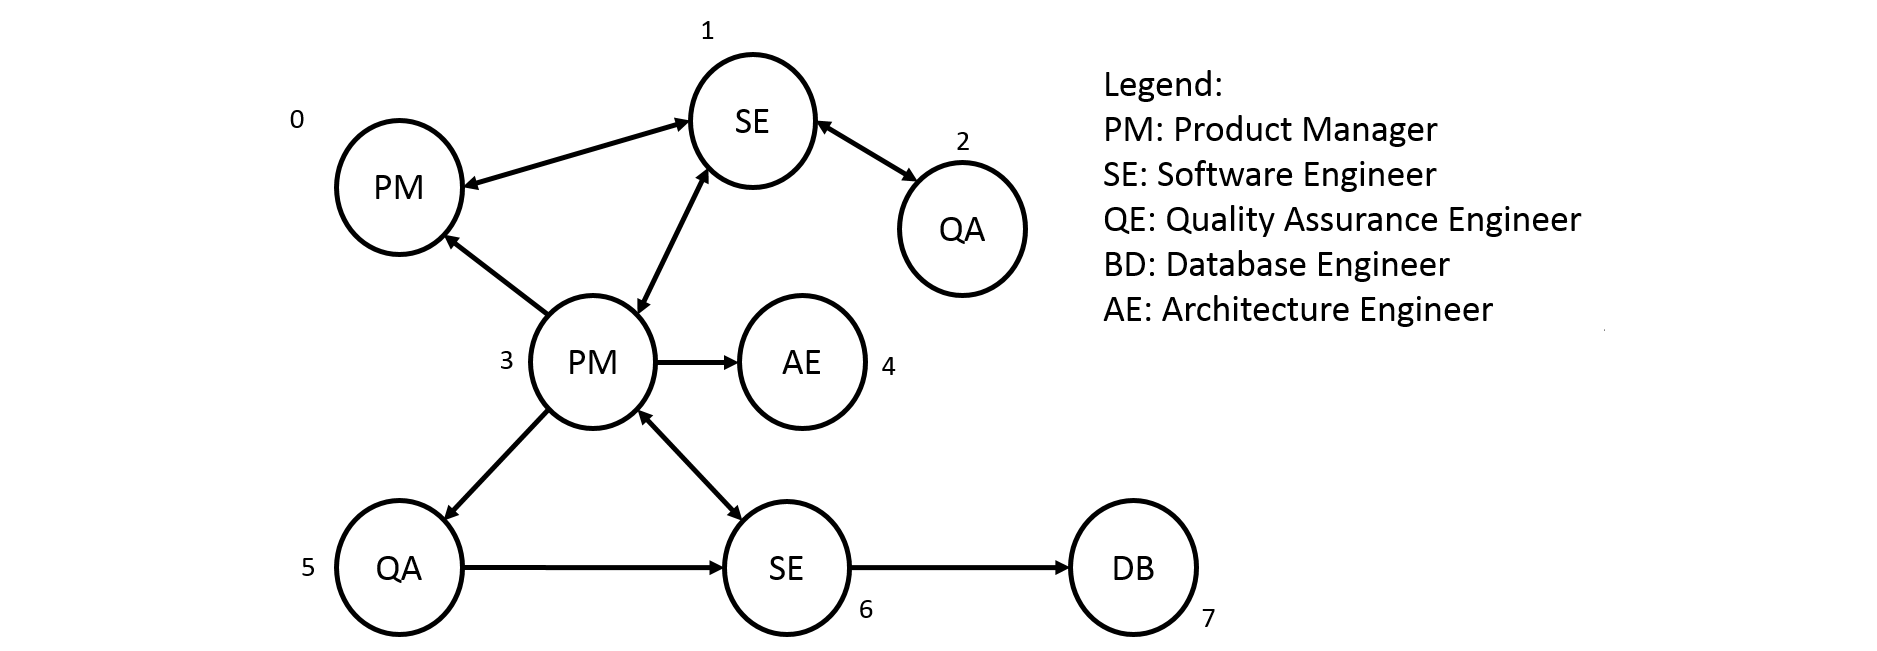
\includegraphics[width=\textwidth]{DataGraph.png}
    \caption{Typed graph with semantics}
    \label{fig:TypedDataGraphExample}
  \end{center}
\end{figure}

\textbf{Structual and semantic matching}

As graph can be either typed or untyped, some pattern matching algorithms are merely based on link structure of the graph and ignore the semantics of the graph. However, some pattern matching algorithms consider the semantics associated with typed vertices/edges of the graph as well as structure. 

\textbf{Exact and inexact matching}

Generally, pattern matching algorithms search subgraphs based on a specified pattern, and the results that match the pattern are in the same shape and have same semantics. This is the exact matching. However, in some situation, the pattern is partially specified, which is inexact matching (e.g. "find all triangle by ignoring the in/out edges"). Even the algorithms find the results that exactly match the pattern, but the results may be in different shape or have different semantics.

\textbf{Exact and approximate solutions}

Pattern matching algorithms vary on whether they guarantee the quality of the results they give. Algorithms for subgraph isomorphism guarantee the results to be optimal solution, if any, but they have been shown with an exponential worst-case complexity. Some algorithms give approximate results by loosing some constrains on the matching criteria, which are often with polynomial complexity. \cite{ma2011capturing} argues that graph isomorphism is sometimes to restrictive to catch sensible matches. To overcome this issue and to reduce the complexity, the several graph simulations are discussed, which actually fall into the category of approximate solutions.

\subsection{General Approach to Graph Pattern Matching}

The original subgraph isomorphism problem has been known as NP-complete\cite{gallagher2006matching}, so all known algorithms for subgraph isomorphism have the complexity of non-polynomial to the size of the input graph. Intuitively, a brute-force way of enumeration can be used to solve the problem. The brute-force enumeration procedure is a depth-first tree-search algorithm\cite{ullmann1976algorithm}.

To solve the problem in a reasonable time, many algorithms for subgraph isomorphism pre-process the data graph to filter the promising candidate for the actual matching processing. In \cite{giugno2002graphgrep, gallagher2006matching}, a basic frame is addressed to generalize this kind of approach. The frame consists of three steps: data analysis, candidate selection and matching. 

Pre-processing on the data graph can yield summary information, such as \textit{graph invariants}, which is helpful in data analysis and metadata construction. An invariant is a quantity to describe a graph. If two graphs are isomorphic, they must have the same invariants. Therefore, invariants can be easily used to compared between pattern and data graph to filter out unlikely matches. A canonical graph representation is used by some algorithms to generate invariants\cite{washio2003state}. In addition, some algorithms use statistical data as summary information\cite{getoor2011learning}.

The metadata of the graph directs candidate selection. If the pattern and a subgraph have different invariants or statistical data, it is unnecessary to perform further matching. If a graph are typed, there are lots of information available for candidate selection. For example, if the pattern contains a vertex of the type Product Manager, not every vertex but only the vertices of Product Manager in the graph should be considered as a potential match. The aim of the candidate selection is to provide a subset of data graph that contains all the potential matches for the matching phase.

In the matching phase, algorithms of structural or semantic matching approach are performed on the candidates to find the matches for the pattern.

\subsection{Distributed Graph Pattern Matching}

In recent years, frameworks, such as Pregel and PowerGraph, have been proposed for distributed graph processing. Many algorithms have been designed to fit this vertex-centric programming paradigm. However, as most algorithms for graph pattern matching are computation intensive, few can be performed on those distributed graph processing frameworks. In \cite{fard2013distributed}, a distributed vertex-centric approach is proposed for graph simulations. With the vertex-centric programming model, in contrast to usual graph programming models, an algorithm should be designed from the perspective of each vertex in a graph. This change from the point of view of vertices makes algorithm design more difficult for the problems like pattern matching that need a global overview of a graph.

To the best of our knowledge, no algorithm for subgraph isomorphism has been designed in vertex-centric way that can run on any of those frameworks yet.

\section{An Algorithm for Distributed Subgraph Isomorphism}

\subsection{Problem Formulation}

As the problem of graph pattern matching has many variations, a specific algorithm should describe what exact problem it can solve. An algorithm based on the GAS model of PowerGraph executed by a synchronous engine is proposed and referred to as DSI later to find isomorphic subgraphs in distributed computation. 

To formally define the subgraph isomorphism with semantics, assume that there is a data graph $G=(V, E, l)$ and a pattern $P=(V_p, E_p, l)$, where $l$ is label function on vertice, which assigns a label to a vertex. Subgraph isomorphism is to find subgraph $G_s=(V_s, E_s, l): V_s \subseteq V, E_s \subseteq E \cap (V_s \times V_s)$, so that there exists a bijective map $f_v : V_s \rightarrow V_p$ such that $(v_1, v_2) \in E_s \iff (f_v(v_1), f_v(v_2)) \in E_p$ and $l(v_1) = l(f(v_1))$ hold. We use $f_e$ to denote the bijective map between $E_s$ and $E_p$.

As PowerGraph can accept directed or undirected graph, no multiple edge, no self-loop, types on vertices or edges(or weights on edges) and connected or unconnected graph, DSI can solve the pattern matching problem, in which the data graph can be directed or undirected, can have types on vertices or edges, can be connected or unconnected, but must not have multiple edges or self-loops. DSI can accept the pattern having the same properties as data graph except that the pattern must be connected. This will not lose the generality, because all the connected parts of pattern can be performed on the same data graph, and the combination of the results will give the isomorphic subgraphs of the unconnected pattern.

DSI gives the exact solutions to exact matching, which can solve both structural and semantic matching problems.

\subsection{Algorithm Description}
\label{sec:dsi-des}

DSI thinks as vertex, which means each vertex knows only information of itself and its neighbors other than the whole data graph. The vertices receive, process and send messages, which are potential isomorphic subgraphs. The data types in DSI are data graph, pattern and message.

The pattern consists of vertices, and each vertex has:	
	\begin{itemize}
	\item A unique $ID_p$
	\item A label for typed graph
	\item Knowledge of the topological relation with neighboring vertices, i.e. what is direction of the edge(s) between it and a neighboring vertex
	\end{itemize}
The data graph consists of vertices, and each vertex has:
	\begin{itemize}
	\item A unique $ID_g$
	\item A label for typed graph
	\item Knowledge of the topological relation with neighboring vertices, i.e. what is direction of the edge(s) between it and a neighboring vertex
	\item Knowledge of the whole pattern
	\item Messages to process
	\end{itemize}	
The message has:
	\begin{itemize}
	\item Possible matching vertices pairs between the pattern and the data graph
	\item The source from where the message is sent
	\item A forwarding trace
	\end{itemize}

The idea behind the algorithm is that the messages representing potential matches go through the data graph and are processed by the vertices to find isomorphic subgraphs, as the vertices only have the local knowledge. The algorithm is explained in the fashion of message passing, which is easy to understand and to transform to the GAS model.

At the beginning, each vertex $v_g$ in the data graph generates a message with matching pair for its each possible matching vertex $v_p$ in the pattern, adds itself to the forwarding trace, and sends the messages to all neighbors.

On receiving messages, vertex $v_g$ uses the following operations on each message according to different situations. 
	\begin{itemize}
	\item \textbf{Forward:} If $v_g$ has matched a vertex in the pattern, it can not match any other pattern vertex. However, an updated message that has never been to $v_g$ should be passed to other possible vertices. In this case, if $v_g$ is not in the forwarding trace, then vertex function adds the vertex itself to the forwarding trace, and sends the message to all neighbors.
	\item \textbf{Update (Spawn):} If $v_g$ has not matched any vertex in the pattern and it can match to some neighbor of the vertex in the pattern, which the message source has matched, then for each possible matching vertex $v_p$, vertex function generates a new message based on the old one by adding the matching pair and replacing all IDs in the forwarding trace with the ID of the current vertex $v_g$. In this case, a message may spawn multiple new messages. If all the pattern vertices have been matched already after this operation in a new message, then an isomorphic subgraph has been found. Otherwise the messages are sent to all neighbors.
	\item \textbf{Drop:} In other situations, the message is dropped, because it is hopeless or redundant to find further matching vertex.
	\end{itemize}

The aim of using the forwarding trace is to avoid the out-of-date messages keeping alive infinitely. If a message is updated, it is fresh to every other vertex. The forwarding trace will be cleared and added with the current vertex ID. If a message is not updated, it can be forwarded by a vertex only once. So a message will die when it reaches the vertex that has seen the message. This mechanism guarantees that the algorithm terminates when there is no live message in the data graph.

In term of "match" between a vertex in the pattern and a vertex in the data graph, the criteria can be divided into structural criteria, which are defined in DSI, and semantic criteria, which can be defined differently for different scenarios. The structural criteria are that there is a bijective map from the vertices set of each subgraph to the vertices set of the pattern, and the edges set of a subgragh in the data graph must be the superset of the pattern. That is to say, if $v_g$ matches $v_p$, the adjacent edges of $v_g$ must be the superset of $v_p$'s adjacent edges. When a vertex $v_g$ checks whether it can match any $v_p$ on receiving a message, it is impossible to compare all the adjacent edges, because maybe not all neighboring vertices of $v_p$ in the pattern are matched. The alternative way to solve this problem is that $v_g$ ensures that the part of the adjacent edges between $v_g$ and previously matched vertices in the data graph are the superset of the part of the adjacent edges between $v_p$ and previously matched vertices in the pattern. As this condition is checked every time a new matching pair is added to the message, an isomorphic subgragh, if found, will keep the structural criteria.

DSI expressed in GAS form is shown as Algorithm~\vref{alg:GAS_DSI}. Messages are created or updated within the vertices. Instead of sending, a vertex gathers the messages from all neighbors in the gather phase (line 1-3). The sum operation aggregates all the messages (line 4-5). In the apply phase, the vertex firstly clears all messages of the last superstep (line 7). If the vertex function just starts, it generates a message with matching pair for each possible matching vertex in the pattern and adds itself to the forwarding trace (line 9). Otherwise it processes each gathered message. If the vertex exists in the matching pair and is not in the forwarding trace (line 12-13), \textbf{Forward} operation is used by adding vertex to the forwarding trace (line 14-15). Otherwise, the vertex uses \textbf{Update (Spawn)} operation. For each neighboring pattern vertex of the one that the message source (the last vertex in the forwarding trace) matches (line 18), the vertex compares matching criteria (line 19). If the vertex can match any, it spawns a new message based on the old one, and adds the matching pair and the forwarding trace (line 20-21). If all pattern vertices have been matched, an isomorphic subgraph is found, otherwise the new message is saved for next superstep (line 22-26). In the scatter phase, the vertex activates itself and all neighbors if there exist messages inside it (line 32-37). The reason to activate the vertex itself is to erase all messages even if no neighbor activates the vertex. Otherwise, the out-of-date messages might be gathered in the future iterations.

To execute the algorithm, the synchronous engine is necessary. Since a vertex will clear all its message before processing gathered messages, it should be guaranteed that all its neighbors gather its messages.


	\begin{Algorithmus}[H]
	\label{alg:GAS_DSI}
	\caption{Distributed Subgraph Isomorphism}	
	\begin{algorithmic}[1]
	
	\State //gather\_nbrs: ALL\_NBRS
	\State \textbf{gather}$(D_u, D_{(u,v)}, D_v)$: 
	\State \textbf{return} messages $D_v.ms$
	\newline
	\State \textbf{sum}$(ms_a, ms_b)$: 
	\State \textbf{return} $ms_a \cup ms_b$
	\newline
	\State \textbf{apply}$(D_u, gathered\_ms)$:
	\State $D_u.ms \leftarrow \emptyset$
	\If  {initialization}
		\State $\forall pv \in V_p, l(u)=l(pv)$: $D_u.ms \leftarrow D_u.ms \cup m$, where $m.pairs = \{(pv, u)\}$, $m.forwardingtrace = \{u\}$   
	\Else		
		\For	{message $m$ : $gathered\_ms$}
			\If  {$\forall (pu, gu) \in m.pairs, \exists gu: u = gu$}
				\If{$u \notin m.forwardingtrace$}
					\State $m.forwardingtrace \leftarrow m.forwardingtrace \cup \{u\}$ 
					\State $D_u.ms \leftarrow D_u.ms \cup m$
				\EndIf
			\Else
				\For {pattern vertex $pv$ : $f_v(m.forwardingtrace.last).neighbors$}
					\If {$\forall (pu, gu) \in m.pairs, \neg \exists pu: pu = pv$ \textbf{and} $\forall (pu, gu) \in m.pairs: f^{-1}_e(e(pv, pu)) \subseteq e(u,gu) $ \textbf{and} $l(u)=l(pv)$}
						\State $m'.pairs \leftarrow m.pairs \cup (pv,u)$
						\State $m'.forwardingtrace \leftarrow \{u\}$	
						\If {$|m'.pairs| = |V_p|$}
							\State $m'.pairs$ is a subgraph
						\Else
							\State $D_u.ms \leftarrow D_u.ms \cup pm'$
						\EndIf		
					\EndIf
				\EndFor		
			\EndIf
		\EndFor		
	\EndIf	
	\newline
	\State  //scatter\_nbrs: ALL\_NBRS
	\State \textbf{scatter}$(D_u, D_{(u,v)}, D_v)$:
	\If{$D_u.ms \neq \emptyset$}
		\State 	Activate($u$)
		\State 	Activate($v$)
	\EndIf

	\end{algorithmic}	
	\end{Algorithmus}

An example is given here to demonstrate how the algorithm works. Assuming that we are interested in finding a work group from the previous example of a team in a software company. So the pattern of the work group is shown in Figure~\ref{fig:BasicPattern}.

\begin{figure}[H]
  \begin{center}
    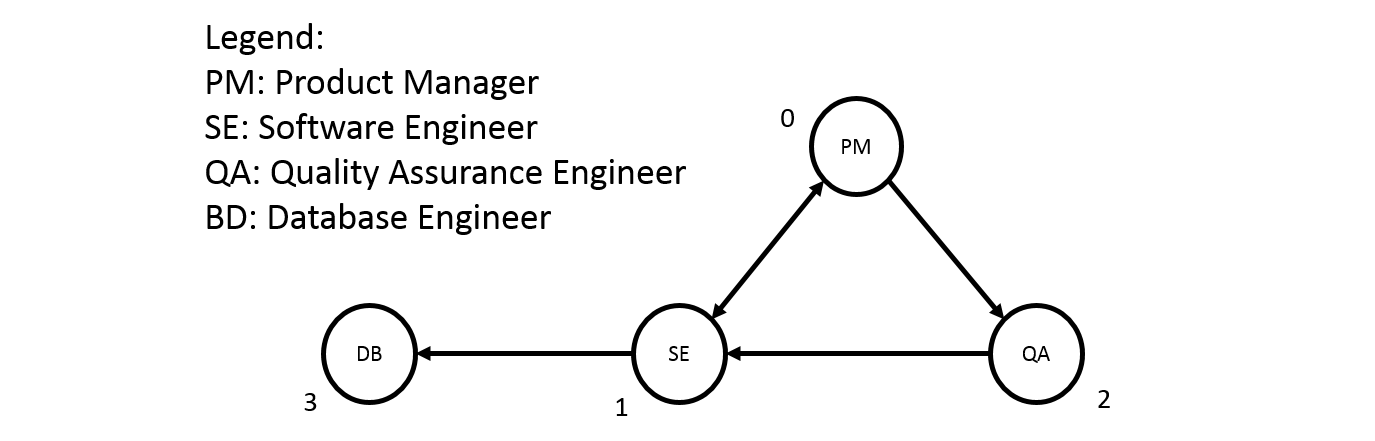
\includegraphics[width=\textwidth]{Pattern.png}
    \caption{Pattern with semantics}
    \label{fig:BasicPattern}
  \end{center}
\end{figure}

To simply and clearly illustrate the procedure of message passing and processing, only one message is created on the vertex 3 and passed through the data graph. The Figure~\ref{fig:MessagePassingDemo} shows the messages in each superstep. A message is denoted as \textbf{(matching IDs)[forwarding trace]}. The initial message (3,-1,-1,-1)[3] means that the data graph vertex 3 has matched to the pattern vertex 0, which is the position in the message. -1 in the message denotes that the pattern vertex has not been matched yet. And the data graph vertex 3 is in the forwarding trace. The message (3,-1,-1,-1)[3] is sent to all the neighboring vertices 0, 1, 4, 5 and 6.  The vertices 0 and 4 can not match any pattern vertex due to the semantic constrain, so they just simply drop the message. When vertex 5 receives the message (3,-1,-1,-1)[3], it checks the matching criteria, and it can match the pattern vertex 2, so it updates the message to (3,-1,5,-1)[5]. This updated message is also sent to all the neighboring vertices including vertex 3. In this case, vertex 3 only adds itself to the forwarding trace and the message becomes (3,-1,5,-1)[5,3]. When vertex 5 receives this message, it finds it is already in the message and the forwarding trace, so the message is dropped. Another example that violates the structural criteria is like this, when vertex 2 receives the message (3,1,-1,-1)[1], it tries to match the pattern vertex 2. However, it cannot keep the topological relation between pattern vertex 0 and 2, so it fails to match and drops the message. Some subgraphs are found in the vertices 5 and 7, which are actually duplicated.

\begin{figure}[H]
  \begin{center}
    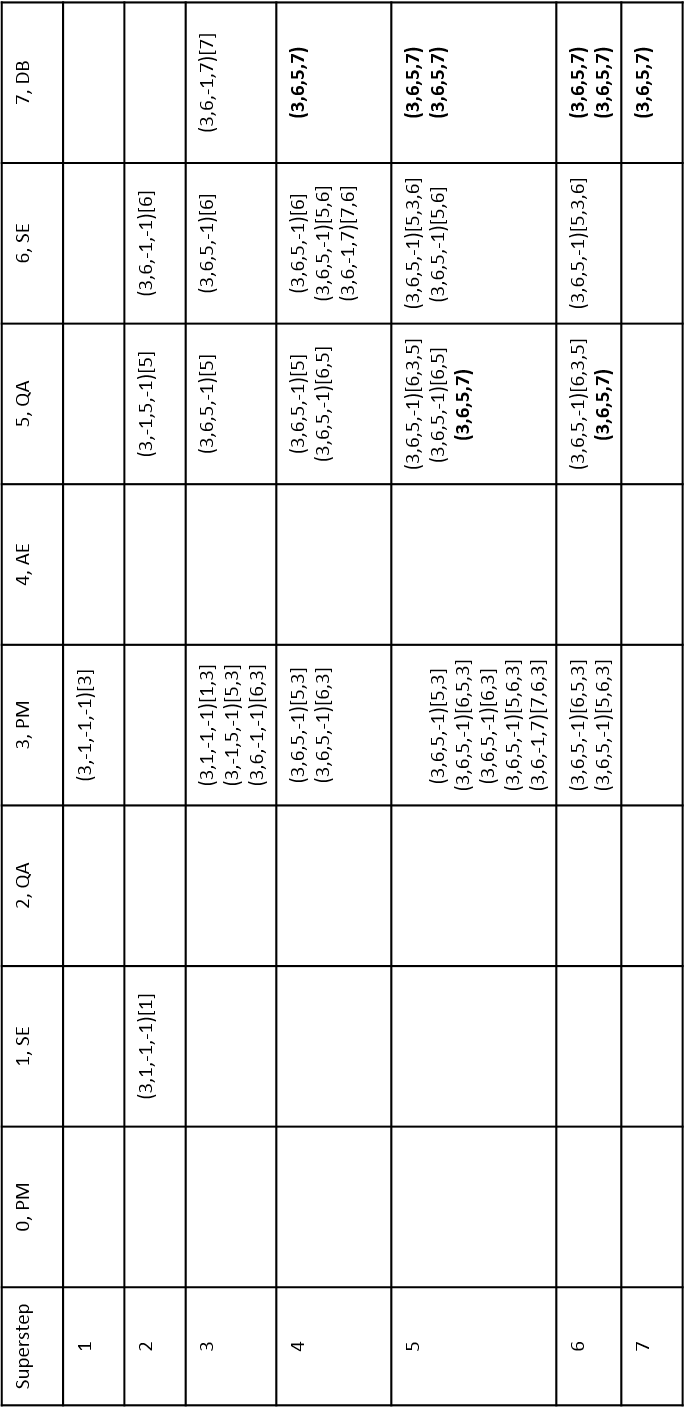
\includegraphics[width=0.64\textwidth]{MessagePassingTable.png}
    \caption{Message passing demonstration}
    \label{fig:MessagePassingDemo}
  \end{center}
\end{figure}

\section{Analysis of DSI}
After giving the description of the algorithm, we have to look at some critical properties of DSI. The algorithm must be correct and able to find all the isomorphic subgraphs, which are discussed in respect of correctness and completeness. We also have to make sure that the algorithm will terminate finally in a distributed environment. At last the complexity of DSI is analysed. After that we are able to know what is the bottleneck of DSI and try to make it more efficient.

\subsection{Correctness}

Here we prove that a subgraph found by the DSI satisfies the definition of the subgraph isomorphism.
 
Firstly, DSI guarantees the bijective map of vertices $f_v:V_s \leftrightarrow V_p$ between the subgraph and the pattern, as they have the same number of vertices and one data graph vertex can only match one pattern vertex. Secondly, the structural matching criteria guarantees topological relation between vertices $(v_1, v_2) \in E_s \iff (f_v(v_1), f_v(v_2)) \in E_p$. As the pattern is restricted to connected graph, the message passing mechanism guarantees that the local knowledge of vertices is enough to solve the problem. Finally, the semantic matching criteria guarantees matching pair has the same label $l(v_1) = l(f_v(v_1))$. 

\subsection{Termination and Deterministic}

As the forwarding trace strategy is used to avoid unchanged messages bounce in the graph infinitely, a message is either updated to an isomorphic subgraph finally or dropped when it cannot spread further. Here we show the maximum supersteps that DSI can have depending on the size of the given pattern, which size must be smaller than or equal to the size of data graph. The maximum number of vertices, to which a brand-new message can be passed (only for the first time) or forwarded without adding new matching pair, is the number of matching pairs in the message. It is the same for the maximum number that a brand-new message can walk among the vertices before a new pattern vertex becomes matched. Given a pattern having $k$ vertices, and a brand-new message with $i$ matching pairs, to find the $(i+1)th$ matching pair, the message at most go through $i$ vertices in the data graph. Therefore, the maximum of supersteps is:

\begin{equation}\label{eq:DSIComplexityMaxIteration}
\begin{split}
	S_{max} &= 1 + \sum_{i=1}^{k-1} i\\
			&= 1 + k*(k-1)/2\\
\end{split}
\end{equation}

The creation of the initial message takes one superstep. This is the upper bound of the superstep for a pattern of size $k$. However, the actual number might be lower, as a message can not walk through all the previously matched vertices because of the pattern topology.

The longest way to find a subgraph in the last example is 3 $\rightarrow$ 6 $\rightarrow$ 3 $\rightarrow$ 5 $\rightarrow$ 3 $\rightarrow$ 6 $\rightarrow$ 7, and corresponding message sequence is (3,-1,-1,-1)[3] $\rightarrow$ (3,6,-1,-1)[6] $\rightarrow$ (3,6,-1,-1)[6,3] $\rightarrow$ (3,6,5,-1)[5] $\rightarrow$ (3,6,5,-1)[5,3] $\rightarrow$ (3,6,5,-1)[5,3,6] $\rightarrow$ (3,6,5,7).

When creating initial messages, only semantic criteria has to be fulfilled, as it is not necessary to check the structural criteria for a single vertex. On receiving messages, both structural and semantic criteria are inspected between the current vertex and pattern vertices. When sending messages, the destinations are all neighbors. As creation, modification and transit of messages only depend on the given pattern and data graph, the outcome of DSI is deterministic.

\subsection{Completeness and Duplication}

DSI can find all the isomorphic subgraphs in the data graph. Messages are created and updated with the data graph.	Each message goes through the data graph until either a subgraph is found or the message is dropped. If there is any isomorphic subgraph, some messages will definitely go through it. As the pattern is restricted to a connected graph, we don't need to worry about the combination of the subgraphs.

However, it can be observed that the isomorphic subgraphs found in the ending vertices are highly duplicated. The reason is that some messages walk through different routes but end with the same subgraph, which is subject to only having the local knowledge in a distributed environment.

\subsection{Complexity}

Given a data graph of size $n$ and a pattern of size $k$, in the initial (first) superstep, each vertex tries to match every possible pattern vertex, so at most $k$ messages can be created. In the first superstep, the upper bound of complexity is:

\begin{equation}\label{eq:DSIComplexityInitial}
	T_1(n,k) = n*k
\end{equation}

In the $ith$ superstep, there are at most $n$ active vertices, each of which has at most $n-1$ neighbors. In each vertex, there can be at most $k*(n-1)^{i-1}$ messages to be processed by its neighbors. To process a message, all the previous matched vertices have to be checked, which are at most $(k-1)$. Therefore, in the $ith$ superstep, the upper bound of complexity is:

\begin{equation}\label{eq:DSIComplexityIth}
	T_i(n,k) = n*(n-1)*k*(n-1)^{i-1}*(k-1)
\end{equation}

In equation~\ref{eq:DSIComplexityMaxIteration} we have shown the maximum supersteps that DSI can run. Therefore the upper bound of total complexity is:

\begin{equation} \label{eq:DSIComplexityTotal}
	\begin{split}
		T(n,k) &= n*k + \sum_{i=2}^{1+k*(k-1)/2} n*(n-1)*k*(n-1)^{i-1}*(k-1)\\
		&= n*k*(1+(k-1)*\sum_{i=2}^{1+k*(k-1)/2} (n-1)^{i})\\
		&= n*k*(1+(k-1)*(\frac{(n-1)^2*((n-1)^{k*(k-1)/2}-1)}{n-2}))\\
	\end{split}
\end{equation}

As known already, subgraph isomorphism is a NP-complete problem, which depends both on the size of the input data graph and the pattern. Because we solve the problem in the distributed environment, it is inevitable to add more complexity.

\section{Optimizations}

One reason for that DSI has high complexity is that messages boost so fast while passing. Eliminating impossible or redundant messages without violating the essential properties of DSI will make DSI more efficient. The term \textit{optimized DSI} is used from now on to refer the algorithm with following optimizations.

\subsection{Constrains on Vertex Degree}
The graph invariants, the in and out degree of vertex, can be used to reduce the impossible messages. If the in or out degree of a data graph vertex is less than a pattern vertex, it is impossible to match those two vertices. So comparing the vertex degree is very helpful, when a vertex tries to match a pattern vertex. In this case, we reduce the messages that are not only created in the initialization but also on processing. Although it can not change the theoretical upper bound of complexity, it practically improves the efficiency of the algorithm.

Algorithm~\vref{alg:GAS_DSI_Degree} with constrains on vertex degree is based on the GAS representation of the original DSI. Here we only highlight the optimized part. The vertex function compares the in and out degree at the initialization (line 7) and when trying to add new matching pair (line 10).

	\begin{Algorithmus}[H]
	\label{alg:GAS_DSI_Degree}
	\caption{Optimized DSI on Vertex Degree}	
	\begin{algorithmic}[1]
	\State \textbf{gather}$(D_u, D_{(u,v)}, D_v)$: 
	\State ...
	\newline
	\State \textbf{sum}$(ms_a, ms_b)$: 
	\State ...
	\newline
	\State \textbf{apply}$(D_u, gathered\_ms)$:
	\If  {initialization}
		\State $\forall pv \in V_p, l(u)=l(pv), in-degree(u) \geq in-degree(pu), out-degree(u) \geq out-degree(pu)$: $D_u.ms \leftarrow D_u.ms \cup m$, where $m.pairs = \{(pv, u)\}$, $m.forwardingtrace = \{u\}$   
	\Else	
		\State ...
			\If {$\forall (pu, gu) \in m.pairs, \neg \exists pu: pu = pv$ \textbf{and} $\forall (pu, gu) \in m.pairs: f^{-1}_e(e(pv, pu)) \subseteq e(u,gu)$ \textbf{and} $in-degree(u) \geq in-degree(pu), out-degree(u) \geq out-degree(pu)$ \textbf{and} $l(u)=l(pv)$}
				\State ...
			\EndIf
		\State ...
	\EndIf
	\newline
	\State \textbf{scatter}$(D_u, D_{(u,v)}, D_v)$:
	\State ...

	\end{algorithmic}	
	\end{Algorithmus}

\subsection{Optimization of Initialization}

If we use the naive method to solve the subgraph isomorphism with a brute-force way of enumeration, we can start enumerating from any vertex, which will not effect the final results. It also makes sense that all vertices just try to match only one specific pattern vertex. This specific initial pattern vertex must be identical, which ensures that at least one message is created within each isomorphic subgraph if any. In the previous example, all the vertices may try to match the pattern vertex 3, so only one message is created in vertex 7 and the subgraph (3,6,5,7) will finally be found. It might not work, for instance, when all the vertices except 7 try to match the pattern vertex 3, but vertex 7 tries to match the pattern vertex 0.

As all the isomorphic subgraphs must contain the matching vertex of the specific initial one, the completeness of the algorithm will not be affected and the duplication of the results will be decreased. In this case, we reduce the messages that are created in the initialization and reduce the upper bound of complexity to:

\begin{equation}\label{eq:DSIComplexityOptimized}
	T(n,k) = n*(1+(k-1)*(\frac{(n-1)^2*((n-1)^{k*(k-1)/2}-1)}{n-2}))
\end{equation}


Choosing different initial pattern vertex may lead to different performance, including duplication degree, the number of messages, communication and etc.. 

Algorithm~\vref{alg:GAS_DSI_Initial} with the optimization of initialization is based on the GAS representation of the original DSI. Here we only highlight the optimized part. The vertex function only tries to match an identical vertex at initialization (line 8).

	\begin{Algorithmus}[H]
	\label{alg:GAS_DSI_Initial}
	\caption{Optimized DSI on Initialization}	
	\begin{algorithmic}[1]
	\State \textbf{gather}$(D_u, D_{(u,v)}, D_v)$: 
	\State ...
	\newline
	\State \textbf{sum}$(ms_a, ms_b)$:
	\State ...
	\newline
	\State \textbf{apply}$(D_u, gathered\_ms)$:
	\State $D_u.ms \leftarrow \emptyset$
	\If  {initialization}
		\State Select an identical $pv \in V_p, l(u)=l(pv)$: $D_u.ms \leftarrow D_u.ms \cup m$, where $m.pairs = \{(pv, u)\}$, $m.forwardingtrace = \{u\}$
	\State ...
	\EndIf
	\newline
	\State \textbf{scatter}$(D_u, D_{(u,v)}, D_v)$:
	\State ...
	\end{algorithmic}	
	\end{Algorithmus}
	
The GAS representation of the optimized DSI is easily deduced by merging the conditions of optimizations. 

\section{Balance Between Algorithm Complexity and Completeness}

The subgraph isomorphism problem is well known as a NP-complete problem and  algorithms for finding isomorphic subgraphs are exponential in
the size of the input graphs. Having exponential complexity, algorithms can not give results within an acceptable time and also might exhaust computing resource when processing large graphs. Sometimes an algorithm that gives a compromising solution with polynomial time complexity is desired, so that the execution time and the resource consumption are guaranteed. Alternatives are approximate solutions with polynomial time complexity, which are not guaranteed to find isomorphic subgraphs.

\subsection{Proportional Distributed Subgraph Isomorphism}

As we observe that in the equation~\ref{eq:DSIComplexityIth}, the upper bound of messages grows theoretically by multiplying $N-1$ after each superstep. We can turn the original solution into an approximate solution with polynomial time complexity, if we can make the factor to a constance. An alternative is proposed here called Proportional Distributed Subgraph Isomorphism (PDSI), which makes compromise between complexity and completeness. Based on the optimized DSI, PDSI differs in that the vertex function only randomly gathers a subset of messages in each neighboring vertex. Therefore, the complexity of the algorithm is significantly reduced. 

PDSI in GAS form is shown in Algorithm~\vref{alg:GAS_PDSI}. We only highlight the part that is modified. The vertex function only randomly gathers a subset of messages in each neighboring vertex (line 2).

	\begin{Algorithmus}[H]
	\label{alg:GAS_PDSI}
	\caption{Proportional Distributed Subgraph Isomorphism}	
	\begin{algorithmic}[1]
	\State \textbf{gather}$(D_u, D_{(u,v)}, D_v)$: 
	\State \textbf{return} Partial message set $ms'$, where $ms' \subseteq D_v.ms$ and $|ms'| = |D_v.ms|*p$, $p \in [0,1]$ is the proportion.
	\newline
	\State \textbf{sum}$(ms_a, ms_b)$:
	\State ...
	\newline
	\State \textbf{apply}$(D_u, gathered\_ms)$:
	\State ...
	\newline
	\State \textbf{scatter}$(D_u, D_{(u,v)}, D_v)$:
	\State ...

	\end{algorithmic}	
	\end{Algorithmus}

%In practice, we can not know \textbf{TODO}

\subsection{Properties of PDSI}

The subgraphs found by PDSI, if any, are still isomorphic to the given pattern, since we don't change the matching criteria. The theoretical upper bound of supersteps is not changed either. But PDSI is not guaranteed to find isomorphic subgraphs, because the necessary routes might not be traversed, which has another effect that the redundant messages are reduced as well.

The parameter $p$ is introduced to denote the proportion of the messages to be gathered in a neighboring vertex. In the $ith$ superstep, there are in total at most $n*(p*(n-1))^i*(k-1)$ messages to be processed. Therefore the upper bound of  the complexity is:

\begin{equation}\label{eq:PDSIComplexity}
	\begin{split}
		T(n,k,p) &= n*(1+(k-1)*\sum_{i=2}^{1+k*(k-1)/2} (p*(n-1))^{i})\\
		&= n*(1+(k-1)*(\frac{(p*(n-1))^2*((p*(n-1))^{k*(k-1)/2}-1)}{n-2}))\\
	\end{split}
\end{equation}

\section{Implementation}

In this section, we give more details about how the proposed algorithms are implemented in PowerGraph. The only essential methods and attributes for algorithms are listed. Functions such as \textit{save()} and \textit{load()}, which are necessary for serialization in PowerGraph are not listed.

The original DSI, optimized DSI and PDSI share the data types in Pattern Vertex, Data Graph Vertex and Message, while they differ in GAS functions.

\subsection{Pattern Vertex}

A pattern vertex should have properties which are mentioned in Section \ref{sec:dsi-des}. The abstract of class PatternVertex is shown in Listing~\ref{lst:PatternVertex}. The attributes are the information of vertex itself and four vectors of neighbors' IDs in different categories. Four methods are used to determine the topological relations between pattern vertices, and then to compare with data graph vertices.

\begin{Listing}[H]
\begin{lstlisting}
class PatternVertex
{
//methods
public:
	bool IsTarget(int id) const;
	bool IsSource(int id) const;
	bool IsNeighbor(int id) const;
	bool IsBi(int id) const;
//attributes
public:
	int id;
	string label;
	unsigned int in_degree;
	unsigned int out_degree;	
	vector<int>	targets;
	vector<int> sources;
	vector<int> neighbors;
	vector<int>	bidirected_neighbors;
};
\end{lstlisting}
\caption{PatternVertex}
\label{lst:PatternVertex}
\end{Listing}

\subsection{Pattern}

The pattern is loaded from a file. User should specify the format of the file and how to interpret. It is also necessary to specify whether the pattern is attributed or not.

\begin{Listing}[H]
\begin{lstlisting}
class Pattern
{
//methods
public:
	bool CreatePattern(string file, bool attributed);
//attributes
public:
	vector<PatternVertex> m_pattern;
};
\end{lstlisting}
\caption{Pattern}
\label{lst:Pattern}
\end{Listing}

\subsection{Message}

A message should store the matching pairs. In practice, we just use a vector to store the data graph vertices ids in a matching order. For example, the vertex, which ID is stored in the first place, matches the first pattern vertex. If a pattern vertex has not been matched yet, -1 is used as a placeholder. A message also has a vector to store the forwarding trace, in which the last one is the message source.

\begin{Listing}[H]
\begin{lstlisting}
typedef std::vector<graphlab::vertex_id_type> IDVector;

class Message
{
//attributes
public:
	IDVector matched_id;
	IDVector forwarding_trace;
};
\end{lstlisting}
\caption{Message}
\label{lst:Message}
\end{Listing}

\subsection{Data Graph Vertex}

A vertex in the data graph is similar to a pattern vertex. In addition, it has more data. The step indicator indicates which stage the vertex function is in. Because in PowerGraph vertex can only directly access the data in adjacent edges, so we use an additional superstep \textit{GetReady} to gather the IDs of the neighboring vertices. \textit{FirstStep} indicates the initialization stage and \textit{SecondStep} is the stage of message processing. Each vertex also contains a local copy of the pattern. The \textit{messages\_in\_vertex} is used to store the messages and the \textit{matched\_subgraphs} stores the isomorphic subgraphs. 

\begin{Listing}[H]
\begin{lstlisting}
enum StepIndicator {GetReady = 0, FirstStep, SecondStep};

class DataGraphVertex
{
//methods
public:	
	bool IsTarget(graphlab::vertex_id_type id) const;
	bool IsSource(graphlab::vertex_id_type id) const;
	bool IsNeighbor(graphlab::vertex_id_type id) const;
	bool IsBi(graphlab::vertex_id_type id) const;
//attributes
public:
	string label;
	Pattern local_pattern;
	StepIndicator si;
	MessagesInVertex messages_in_vertex;
	vector<IDVector> matched_subgraphs;	
	IDVector	targets;
	IDVector 	sources;
	IDVector 	neighbors;
	IDVector	bidirected_neighbors;
};
\end{lstlisting}
\caption{DataGraphVertex}
\label{lst:DataGraphVertex}
\end{Listing}

%\subsection{GAS Functions}